\documentclass[../main.tex]{subfiles}
\begin{document}
\chapter{Line, Area, Surface, and Volume Integrals}
\section{Line Integrals}
\subsection{Definitions}
\begin{definition}
  Given a curve $C$ parameterised by $t \in [a, b]$, the \textit{line integral} of a vector field $\vec{F}$ along $C$ is:
  \[
    \int_{C} \vec{F} \cdot \d{\vec{x}} = \int_{a}^{b} \vec{F}(\vec{x}(t)) \cdot \deriv{\vec{x}}{t} \d{t}
  \]
\end{definition}
An alternative, but equivalent definition, is to split the curve up at points $\vec{x}_0, \ldots, \vec{x}_n$ on the curve in that order with $\vec{x}_0 = \vec{x}(a)$ and $\vec{x}_N = \vec{x}(b)$.
We then let $\delta \vec{x}_n = \vec{x}_{n + 1} - \vec{x}_n$ for $n \in \{0, \ldots, N - 1\}$.
Then we define the line integral as:
\[
  \int_{C} \vec{F} \cdot \d{\vec{x}} = \lim_{\Delta \to 0} \sum_{n = 0}^{N-1} \vec{F}(\vec{x}_n) \cdot \delta \vec{x}_n
\]
where $\Delta = \max\limits_{0 \leq n \leq N - 1}|\delta \vec{x}_n|$.
Note that as $\Delta \to 0$, we must have $N \to \infty$ so that we still cover the whole curve.
\begin{remark}
  Less commonly, other types of line integral can also be used.
  For example:
  \[
    \int_{C} f(\vec{x}) \d{s} = \int_{a}^{b} f(\vec{x}(t))\abs{\deriv{\vec{x}}{t}} \d{t}
  \]
  as $\deriv{s}{t} = \abs{\deriv{\vec{x}}{t}}$ from \cref{arcLength}.

  Or:
  \[
    \int_{C} \vec{F} \times \d{\vec{x}} = \int_{a}^{b} \vec{F}(\vec{x}(t)) \times \deriv{\vec{x}}{t} \d{t}
  \]
\end{remark}
\begin{remark}[Dynamics and Relativity]
  We saw in Dynamics and Relativity that if $\vec{F}$ is a force being applied to a particle at $\vec{x}(t)$, then $\int_{C} \vec{F} \cdot \d{\vec{x}}$ is called the \textit{work done} by the force along $C$.
\end{remark}
\begin{definition}[Circulation]
If $C$ is a closed curve, then the line integral around the whole curve is denoted:
\[
  \oint_C \vec{F} \cdot \d{\vec{x}}
\]
which is sometimes known as \textit{circulation} of $\vec{F}$ around $C$.
\end{definition}
\begin{remark}
  It does not matter where we start a line integral over a closed loop, provided that we go all the way around.
\end{remark}
We can reverse line integrals using:
\[
  \int_{-C} \vec{F} \cdot \d{\vec{x}} = - \int_{C} \vec{F} \cdot \d{\vec{x}}
\]
and split them up using:
\[
  \int_{C_1 + C_2} \vec{F} \cdot \d{\vec{x}} = \int_{C_1} \vec{F} \cdot \d{\vec{x}} + \int_{C_2} \vec{F} \cdot \d{\vec{x}}
\]
\subsection{Examples}
\begin{example}[Examples of Line Integrals]
  \label{lineIntegralExamples}
  \begin{enumerate}
    \item Integrate $\vec{F} = (y, -x, 0)$ on the straight line $C_1$ joining $(-1, 0, 0)$ and $(1, 0, 0)$.

      We can parametrise the curve as $\vec{x} = (t, 0, 0)$ for $t \in [-1, 1]$.
      Then:
      \[
        \vec{F}(\vec{x}(t)) = (0, -t, 0) \text{ and } \dot{\vec{x}} = (1, 0, 0)
      \]
      so
      \[
        \int_{C_1} \vec{F} \cdot \d{\vec{x}} = \int_{C_1} \vec{0} \cdot \d{\vec{x}} = 0
      \]
    \item Integrate $\vec{F} = (3x^2, 2y, 0)$ on $C_1$.

      We have:
      \[
        \vec{F} \cdot \dot{\vec{x}} = (3t^2, 0, 0) \cdot (1, 0, 0) = (3t^2, 0, 0)
      \]
      so:
      \[
        \int_{C_1} \vec{F} \cdot \d{\vec{x}} = \int_{-1}^{1} 3t^2 \d{t} = \eval{x^3}{-1}{1} = 2
      \]
    \item Integrate $\vec{F} = (y, -x, 0)$ along the curve $C_2$ joining $(-1, 0, 0)$ to $(1, 0, 0)$ parameterised by $\vec{x} = (t - 1, t(t - 2), t(t^2 - 4))$ for $t \in [0, 2]$.

      We have:
      \[
        \vec{F} = (t(t - 2), 1 - t, 0) \text{ and } \dot{\vec{x}} = (1, 2t - 2, 3t^2 - 4)
      \]
      so:
      \[
        \int_{C_2} \vec{F} \cdot \d{\vec{x}} = \int_{0}^{2} (t(t - 2) - 2(t - 1)^2) \d{t} = \eval{-\frac{1}{3}t^3 + t^2 - 2t}{0}{2} = -\frac{8}{3}
      \]
    \item Integrate $\vec{F} = (3x^2, 2y, 0)$ on $C_2$.

      We have:
      \begin{align*}
        \vec{F} \cdot \dot{\vec{x}} &= (3(t - 1)^2, 2t(t - 2), 0) \cdot (1, 2t - 2, 3t^2 - 4) \\
                                    &= 4t^3 - 9t^2 + 2t + 3
      \end{align*}
      so:
      \[
        \int_{C_2} \vec{F} \cdot \d{\vec{x}} = \int_{0}^{2} 4t^3 - 9t^2 + 2t + 3 \d{t} = \eval{t^4 - 3t^3 + t^2 + 3t}{0}{2} = 2
      \]
    \item What is the work done by a force field $\vec{F} = (y^2 e^{x}, e^{y} + 2ye^{x}, 0)$ moving a particle along $C_3$, which is the ellipse $x^2/a^2 + y^2/b^2 = 1$ in the $x$-$y$ plane starting at $(a, 0, 0)$ and going anticlockwise to $(0, b, 0)$.

      We can parametrise this ellipse as $\vec{x}(\theta) = (a \cos \theta, b \sin \theta, 0)$ for $\theta \in [0, \frac{\pi}{2}]$.
      We then have:
      \[
        \vec{F}(\vec{x}(\theta)) = (b^2 \sin^2 \theta e^{a \cos \theta}, e^{b \sin \theta} + 2b\sin\theta e^{a \cos \theta}, 0)
      \]
      and:
      \[
        \deriv{\vec{x}}{\theta} = (-a \sin \theta, b \cos \theta, 0)
      \]
      so:
      \[
        \vec{F} \cdot \deriv{\vec{x}}{\theta} = -ab^2 \sin^3 \theta e^{a \cos \theta} + b \cos \theta e^{b \sin \theta} + 2b^2 \sin \theta \cos \theta e^{a \cos \theta}
      \]
      We can now evaluate the integral:
      \begin{align*}
        \int_{C_3} \vec{F} \cdot \d{\vec{x}} &= \eval{e^{b \sin \theta}}{0}{\pi/2} + \int_{0}^{\pi/2} b^2 \sin \theta e^{a \cos \theta} (-a + 2\cos \theta + a \cos^2 \theta) \d{\theta} \\
                                             &= e^{b} - 1 + \int_{1}^{0} b^2e^{ai}(1 - 2u - au^2) \d{u} \text{ using $u = \cos \theta$}\\
                                             &= e^{b} - 1 + \eval{b^2 e^{au}(1 - u^2)}{1}{0} \\
                                             &= e^{b} - 1 + b^2
      \end{align*}
      If we instead went around the whole ellipse, starting at $(a, 0, 0)$ and going anticlockwise all the way around, we would find that $\oint \vec{F} \cdot \d{\vec{x}} = 0$.
    \item We can also integrate along a path parameterised in a different coordinate system, for example, cylindrical polar coordinates (\cref{cylindricalPolar}).

      Integrate $\vec{F} = z \vec{e}_\phi$ on the path $C_4$ given by $\rho = z^2$, $\phi = \pi z$ for $z = 0$ to $z = 1$.

      We know from \cref{cylindricalInfinitesimals} that:
      \[
        \d{\vec{x}} = \d{\rho}\vec{e}_\rho + \rho \d{\phi}\vec{e}_\phi + \d{z}\vec{e}_z
      \]
      so:
      \[
        \d{\vec{x}} = (2z\vec{e}_\rho + \pi \rho \vec{e}_\phi + \vec{e}_z) \d{z}
      \]
      as $\deriv{\rho}{z} = 2z$ and $\deriv{\phi}{z} = \pi$.
      We then have $\vec{F} \cdot \d{\vec{x}} = \pi \rho z \d{z} = \pi z^3 \d{z}$ and so:
      \[
        \int_{C_4} \vec{F} \cdot \d{\vec{x}} = \int_{0}^{1} \pi z^3 \d{z} = \frac{\pi}{4}
      \]
  \end{enumerate}
\end{example}
\subsection{Path Independence}
\begin{definition}[Exact Differential]
  We say that the differential form $\vec{F} \cdot \d{\vec{x}}$ is \textit{exact} if there exists a single valued scalar field $f(\vec{x})$ such that:
  \[
    \vec{F} \cdot \d{\vec{x}} = F_i \d{x_i} = \d{f}
  \]
  for all $\d{\vec{x}}$.
\end{definition}
\begin{remark}[Recap]
  We saw exact differentials in 2D in IA Differential Equations.
\end{remark}
We also know from \cref{infinitesimalsGrad} that $\d{f} = \nabla f \cdot \d{\vec{x}}$ and so $\vec{F} \cdot \d{\vec{x}}$ is exact if and only if there exists a single valued function such that $\vec{F} = \nabla f$, that is, it is exact if and only if $\vec{F}$ is a conservative (\cref{conservativeField}) field.

\begin{proposition}
  If $\vec{F} = \nabla f$ is a conservative vector field and $C$ is a path from $a$ to $b$, then:
  \[
    \int_{C} \vec{F} \cdot \d{\vec{x}} = f(\vec{b}) - f(\vec{a})
  \]
  So the line integral depends only on the endpoints of the path.
\end{proposition}
\begin{proof}
  We can write $\vec{F} = \nabla f$ and so $\d{f} = \nabla f \cdot \d{\vec{x}} = \vec{F} \cdot \d{\vec{x}}$.
  Substituting this into the integral:
  \[
    \int_{C} \vec{F} \cdot \d{\vec{x}} = \int_{C} \d{f} = \eval{f}{\vec{a}}{\vec{b}} = f(\vec{b}) - f(\vec{a})
  \]
\end{proof}
\begin{proof}[Alternative]
Since $\deriv{f}{t} = \dot{\vec{x}} \cdot \nabla f$ from \cref{MVCGrad}, we have:
\[
  \int_{C} \vec{F} \cdot \d{\vec{x}} = \int_{C} \nabla f \cdot \dot{\vec{x}} \d{t} = \int \deriv{f}{t} \d{t} = f(\vec{b}) - f(\vec{a})
\]
\end{proof}
\begin{remark}[Notation]
  Since the value of the line integral is independent of the particular path $C$ between $\vec{a}$ and $\vec{b}$, we can write  $\int_{\vec{a}}^{\vec{b}} \vec{F} \cdot \d{\vec{x}}$ without ambiguity.
  We usually would not be able to do this as different paths would result in different values, hence why we usually specific a path $C$.
\end{remark}
\begin{corollary}
  If $\vec{F}$ is conservative and $C$ is a closed curve, then $\oint_C \vec{F} \cdot \d{\vec{x}} = 0$.
\end{corollary}
\begin{proof}
  Since $\vec{F}$ is conservative, we can write $F = \nabla f$ for a \textbf{single valued} $f$.
  The curve is closed so the value of the integral is $f(\vec{a}) - f(\vec{a})$ which is zero since $f$ is single valued.
\end{proof}
\begin{proposition}
  In a \textbf{simply connected domain}, the following are equivalent:
  \begin{enumerate}
    \item $\vec{F}$ is a conservative vector field.
    \item There exists a single valued $f(\vec{x})$ such that $\vec{F} = \nabla f$.
    \item $\vec{F} \cdot \d{\vec{x}}$ is an exact differential.
    \item $\vec{F}$ is irrotational.
    \item $\nabla \times \vec{F} = \vec{0}$.
    \item $\pderiv{F_i}{x_j} = \pderiv{F_j}{x_i}$ for all $i, j$
    \item For any $\vec{a}, \vec{b}$ in the domain of $\vec{F}$, $\int_{\vec{a}}^{\vec{b}} \vec{F} \cdot \d{\vec{x}}$ is path independent.
    \item $\oint_C \vec{F} \cdot \d{\vec{x}} = 0$ for all closed curves $C$ in the domain.
  \end{enumerate}
\end{proposition}
\begin{proof}
  \begin{itemize}
    \item \textbf{i} $\iff$ \textbf{ii} and \textbf{iv} $\iff$ \textbf{v} by definition.
    \item \textbf{i} $\iff$ \textbf{iii} was shown above.
    \item \textbf{i} $\iff$ \textbf{iv}, see \cref{conservativeFields}.
    \item \textbf{v} $\iff$ \textbf{vi} by considering components of $\nabla \times \vec{F}$:
      \[
        [\nabla \times \vec{F}]_k = \levi_{i j k} \pderiv{F_j}{x_i} = 0
      \]
      which is true for all $k$ if and only if $\pderiv{F_j}{x_i}$ is symmetric in $i$ and $j$.
    \item \textbf{ii} $\implies$ \textbf{vii} was shown above.
    \item \textbf{vii} $\implies$ \textbf{viii}, given any closed curve $C$ we can split it into two parts, $C_1$ from $\vec{a}$ to $\vec{b}$, then $C_2$ from $\vec{b}$ back to $\vec{a}$ so that $C = C_1 + C_2$, but, by assumption, since $C_1$ and $-C_2$ have the same endpoints:
      \[
        \int_{C_1} \vec{F} \cdot \d{\vec{x}} = \int_{-C_2} \vec{F} \cdot \d{\vec{x}} = - \int_{C_2} \vec{F} \cdot \d{\vec{x}}
      \]
      and so:
      \[
        \oint_C \vec{F} \cdot \d{\vec{x}} = \int_{C_1} \vec{F} \cdot \d{\vec{x}} + \int_{C_2} \vec{F} \cdot \d{\vec{x}} = 0
      \]
  \end{itemize}
  This leaves \textbf{viii} $\implies$ \textbf{vii} and \textbf{vii} $\implies$ \textbf{ii} which will be proved in the next chapter in \cref{scalarPotentials}.
\end{proof}
\begin{example}[Revisiting \cref{lineIntegralExamples}]
  \begin{itemize}
    \item In \textbf{i} and \textbf{iii}, we integrated $\vec{F} = (y, -x, 0)$ along two different paths.
      We see that $\vec{F}$ is not conservative as $\nabla \times \vec{F} = (0, 0, -2) \neq \vec{0}$.
      This agrees with how we got two different values for the line integral on the two different paths, despite the fact that they had the same end points.
    \item In \textbf{ii} and \textbf{iv} we integrated $\vec{F} = (3x^2, 2y, 0)$ along two different paths.
      Here $\vec{F}$ is conservative as $\nabla \times \vec{F} = \vec{0}$.
      We can also just spot that $\vec{F} = \nabla (x^3 + y^2)$, and so it follows that $\vec{F}$ is conservative as it has a single valued scalar potential.

      Therefore the value of the integral is path independent so:
      \[
        \int_{(-1, 0, 0)}^{(1, 0, 0)} \vec{F} \cdot \d{\vec{x}} = \eval{x^3 + y^2}{(-1, 0, 0)}{(1, 0, 0)} = 2
      \]
      which agrees with our answers, despite the different paths.
    \item In \textbf{v}, we integrated $\vec{F} = (y^2 e^{x}, e^{y} + 2ye^{x}) = \nabla(e^{y}, y^2e^{x})$ which is conservative and so we can shortcut the rather involved integration to obtain:
      \[
        \int_{C_3} \vec{F} \cdot \d{\vec{x}} = \eval{e^{y} + y^2e^{x}}{(a, 0, 0)}{(0, b, 0)} = e^{b} + b^2 - 1
      \]
      which agrees with our answer.
    \item In \textbf{vi}, we integrated $F = z \vec{e}_\phi$.
      Using \cref{cylindricalOperators}, we see that $\nabla \times (z \vec{e}_\phi) = -\vec{e}_\rho \neq \vec{0}$ and so $\vec{F}$ is not conservative.

      Suppose that $\nabla \times \vec{F}$ had actually been $\vec{0}$, we could not have concluded that $\vec{F}$ would be conservative.
      The domain of $\vec{F}$ does not include the $z$-axis apart from $\vec{0}$ as $\vec{e}_\phi$ is not defined there.
      So we could shrink a curve around the $z$ axis to a point by passing it through the ``gap'' at the origin, however, the derivatives of $F$ are not defined at the origin and so $\nabla \times \vec{F}$ is also not defined there so we are not working in a simply connected domain.
  \end{itemize}
\end{example}
\section{Area Integrals}
\label{areaIntegrals}
\subsection{Definition}
To integrate over a region $A \subset \R^2$, we cover $A$ with a large number $N$ of small disjoint subsets $\delta A_i \subset A$ for $i \in \{1, \ldots, N\}$.
Then:
\[
  \int_A f(x, y) \d{x} = \lim_{\Delta \to 0} \sum_{i = 1}^{N} f(x_i, y_i) \delta A_i
\]
where $(x_i, y_i) \in \delta A_i$ and $\Delta$ is the maximum linear dimension of all the $\delta A_i$, and as $\Delta \to 0$, $N \to \infty$ so that the shrinking subsets still cover the entirety of $A$.

Informally, we can think of $\int_A f(x, y) \d{A}$ is the volume under the graph of $z = f(x, y)$, similarly to how we can think of $\int_{a}^{b} f(x) \d{x}$ as the area under the graph $y = f(x)$.
\begin{remark}[Note]
  $A$ refers to both the region itself and its area so:
  \[
    A = \int_A 1 \d{A}
  \]
\end{remark}
\begin{remark}
  It does not matter how we divide $A$ up, every different way will lead to the same answer as $\Delta \to 0$.

  If it doesn't give the same answer, then we say that $f$ is not integrable of $A$ but for most reasonable functions $f$ and regions $A$, it will be integrable.
\end{remark}
The most obvious way to divide $A$ up is to use rectangles parallel to the $x$ and $y$ axes with area $\delta x \delta y$.

If we first sum over a horizontal strip of $y$ with constant height $\delta y$ and let $\delta x \to 0$ then we obtain:
\[
  \left(\int_{X(y)} f(x, y) \d{x}\right)\delta y
\]
where for each $y$, $X(y) = \{x: (x, y) \in A\}$.
We then sum these over the range of $y$ and let $\delta y \to 0$ to obtain:
\[
  \int_{y_{\text{min}}}^{y_{\text{max}}} \left(\int_{X(y)} f(x, y) \d{x}\right) \d{y}
\]

We could also sum vertical strips to obtain:
\[
  \int_{x_{\text{min}}}^{x^{\text{max}}} \left(\int_{Y(x)} f(x, y) \d{y}\right) \d{x}
\]
where $Y(x) = \{y: (x, y) \in A\}$.

\textit{Fubini's Theorem} tells us that both of these are equal to $\int_A f(x, y) \d{A}$ for any reasonable $f$ and $A$.
That is, taking the limits in $x$ and then $y$, is the same as taking the limits in $y$ and then $x$, and the same as taking $\Delta \to 0$.
\begin{remark}[Restrictions on Fubini's Theorem]
  \nonexaminable
  When we mean reasonable $f$ and $A$, the restrictions are quite loose, if $f$ is piecewise continuous and the boundary of $A$ is a finite piecewise smooth curve then Fubini's Theorem holds.
\end{remark}
\begin{remark}[Notation]
  Some other notation for $\int_A f(x, y) \d{A}$  include:
  \[
    \int_A f(x, y) \d{x} \d{y},\ \int_A f(\vec{x}) \d^2{\vec{x}},\ \iint\limits_A f(x, y) \d{A},\ \int_A f(x, y) \d{S},\ \int\d{x}\int\d{y} f(x, y)
  \]
\end{remark}
\begin{example}
  Integrate $f(x, y) = xy^2$ over $A$, a triangle with vertices at $(0, 0), (1, 1)$ and $(1, -1)$.

  \begin{center}
  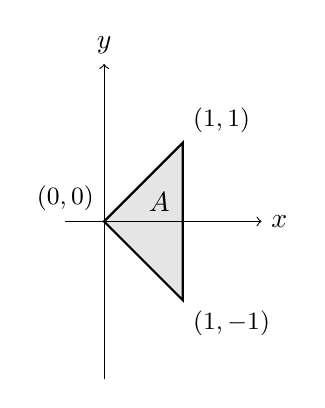
\begin{tikzpicture}
    \filldraw[fill=gray!20, draw=black, thick] (0, 0) node[above left] {\small$(0, 0)$} -- (1, 1) node[above right] {\small$(1, 1)$} -- (1, -1) node[below right] {\small$(1, -1)$} -- cycle;
    \node[above] at (0.7, 0) {$A$};
    \draw[->] (-0.5, 0) -- (2, 0) node[right] {$x$};
    \draw[->] (0, -2) -- (0, 2) node[above] {$y$};
  \end{tikzpicture}
  \end{center}

  We can integrate over $y$ first:
  \begin{align*}
    \int_A f(x, y) \d{A} &= \int_{0}^{1} \int_{-x}^{x} xy^2 \d{y} \d{x} \\
                         &= \int_{0}^{1} x \eval{\frac{1}{3} y^3}{-x}{x} \d{x} \\
                         &= \int_{0}^{1} \frac{2}{3}x^{4} \d{x} \\
                         &= \frac{2}{15}
  \end{align*}
  We can also integrate over $x$ first, although the bounds are a bit more fiddly:
  \begin{align*}
    \int_A f(x, y) \d{A} &= \int_{-1}^{1} \int_{|y|}^{1} xy^2 \d{x} \d{y} \\
                         &= \int_{-1}^{1} y^2 \eval{\frac{1}{2}x^2}{|y|}{1} \d{y} \\
                         &= \int_{-1}^{1} \frac{1}{2}y^2(1 - y^2) \d{y} \\
                         &= \frac{1}{3} - \frac{1}{5} = \frac{2}{15}
  \end{align*}
\end{example}
\begin{remark}[Warning]
  Make sure that you determine the inner limits in terms of the outer variable.
  A common mistake is to just make both limits run between the min and max of $x$ and $y$, however, this means that you will always be integrating over a rectangle.
\end{remark}
\begin{remark}[Special Case]
  If $A$ is a rectangle, i.e. $A = \{(x, y): x \in [a, b], y \in [c, d]\}$, and $f$ is \textit{separable} so it can be written as $f(x, y) = g(x)h(y)$, then we can do the $x$-integral first, pulling out $h(y)$:
  \[
    \int_{X(y)} f(x, y) \d{x} = h(y) \int_{a}^{b} g(x) \d{x}
  \]
  Now when we do the outer integral, $\int_{a}^{b} g(x) \d{x}$ is just a constant so can be pulled out so:
  \[
    \int_A f(x, y) \d{A} = \left(\int_{a}^{b} g(x) \d{x}\right)\left(\int_{c}^{d} h(y) \d{y}\right)
  \]
\end{remark}
\subsection{Change of Variables and the Jacobian}
\begin{proposition}[Change of variables for area integrals]
  If $(u, v) \mapsto (x, y)$ is a bijection (apart from perhaps at a set of points with measure zero) from a region $A'$ in the $(u, v)$-plane to the region $A$ in the $(x, y)$-plane, then:
  \label{areaCoV}
  \[
    \int_A f(x, y) \d{x} \d{y} = \int_{A'} F(u, v) \abs{\frac{\partial(x, y)}{\partial(u, v)}} \d{u}\d{v}
  \]
  where $F(u, v) = f(x(u, v), y(u, v))$ and:
  \[
    J = \frac{\partial(x, y)}{\partial(u, v)} \equiv \det \begin{pmatrix}
    \pderiv{x}{u} & \pderiv{x}{v} \\
    \pderiv{y}{u} & \pderiv{y}{v} \\
    \end{pmatrix}
  \]
  is called the \textit{Jacobian} of the transformation.
\end{proposition}
\begin{remark}[Note]
  It is the \textbf{modulus} of $J = \frac{\partial(x, y)}{\partial(u, v)}$ that appears in this rule, not a determinant.
  That is, we have a factor of $|J|$ where $J$ is the \textbf{determinant} of a matrix.
\end{remark}
\begin{remark}[Notation]
  We often just call $F$ just $f$ so the right hand side reads:
  \[
    \int_{A'} f(u, v) |J| \d{u} \d{v}
  \]
  which is clearly incorrect but regardless it is usually clear what is meant.
\end{remark}
\begin{proof}
  We can choose how we want to divide $A$ up and so we choose to divide $A$ up into small regions between curves of constant $u$ and constant $v$.
  In \cref{surfaceElements}, we saw how we can find the area of such a region on a 2D surface, so, as we can consider $A$ a flat surface in the $(x, y)$-plane, the area of each region is given by:
  \[
    \abs{\pderiv{\vec{x}}{u} \times \pderiv{\vec{x}}{v}} \d{u} \d{v} = \abs{\begin{pmatrix}
    \pderiv{x}{u} \\
    \pderiv{y}{u} \\
    0 \\
    \end{pmatrix} \times \begin{pmatrix}
    \pderiv{x}{v} \\
    \pderiv{y}{v} \\
    0 \\
    \end{pmatrix}} \d{u} \d{v} =
    \abs{\pderiv{x}{u}\pderiv{y}{v} - \pderiv{x}{v}\pderiv{y}{u}}\d{u}\d{v} = |J| \d{u}\d{v}
  \]
  The contribution of this particular region to the sum defining $\int_A f \d{A}$ is therefore $f(\vec{x}(u, v))|J| \d{u} \d{v} = F(u, v) |J| \d{u} \d{v}$.
  Integrating over the values of $(u, v) \in A'$, we have:
  \[
    \int_A f \d{x} \d{y} = \int_{A'} F |J|\d{u} \d{v}
  \]
\end{proof}
\begin{remark}
  The goal of using such a transform is either to simplify the region of integration and/or the integrand.
\end{remark}
\begin{example}
  Evaluate the integral $\int_A y^2 \d{A}$ where $A$ is the semicircular domain $\{(x, y): x^2 + y^2 < R^2,\ y > 0\}$.

  We choose plane polar coordinates $(r, \theta)$ defined by $x = r\cos \theta$, $y = r\sin\theta$.
  Then in the $(r, \theta)$-plane, we see that there is a bijection between the rectangle $A' = \{(r, \theta): r < R,\ 0 < \theta < \pi\}$ and $A$.

  We first find the Jacobian of the transformation:
  \[
    |J| = \det \begin{pmatrix}
    \pderiv{x}{r} & \pderiv{x}{\theta} \\
    \pderiv{y}{r} & \pderiv{y}{\theta} \\
    \end{pmatrix} = \det \begin{pmatrix}
    \cos \theta & -r\sin \theta \\
    \sin \theta & r\cos \theta \\
    \end{pmatrix} = r
  \]
  We also find that $F(r, \theta) = f(r \cos \theta, r \sin \theta) = r^2 \sin^2 \theta$ and so:
  \[
    \int_A y^2 \d{A} = \int_{A'} r^2 \sin^2 \theta |r| \d{r} \d{\theta}
  \]
  Since $F$ separable and we are integrating over the rectangle $A'$, we obtain:
  \[
    \int_{0}^{R} r^3 \d{r} \int_{0}^{\pi} \sin^2\theta \d{\theta} = \frac{1}{8}\pi R^4
  \]

  In this example, the area element was $\d{A'} = r \d{r} \d{\theta}$.
  The curves of constant $r$ are circles radius $r$ and the curves of constant $\theta$ are straight lines:
  \begin{center}
  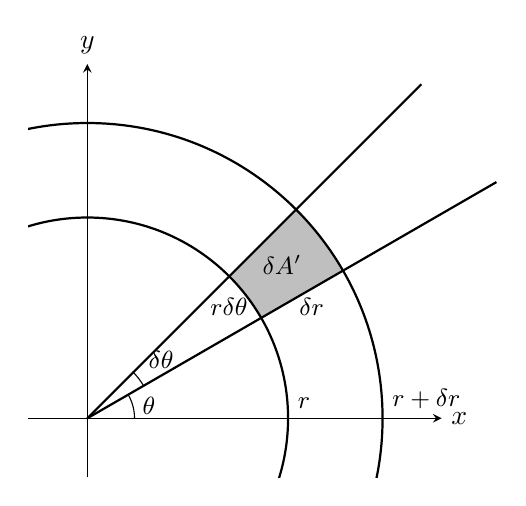
\begin{tikzpicture}[>=stealth, scale=1.5]
    \begin{scope}
      \clip (0, 0) -- (3, 3) -- (2.165, 1.25);
      \fill[gray!50] (0, 0) circle (2.5);
      \fill[white] (0, 0) circle (1.7);
    \end{scope}
    \begin{scope}
      \clip (-0.5, -0.5) rectangle (3, 3);
      \draw[thick] (0, 0) circle (2.5);
      \draw[thick] (0, 0) circle (1.7);
    \end{scope}
    \draw[->] (-0.5, 0) -- (3, 0) node[right] {$x$};
    \draw[->] (0, -0.5) -- (0, 3) node[above] {$y$};
    \draw[rotate = 45, thick] (0, 0) -- (4, 0);
    \draw[rotate = 30, thick] (0, 0) -- (4, 0);
    \node[above right] at (2.5, 0) {\small$r + \delta r$};
    \node[above right] at (1.7, 0) {\small$r$};
    \node[below] at (1.9, 1.1) {\small$\delta r$};
    \node[below] at (1.2, 1.1) {\small$r \delta \theta$};
    \node at (1.65, 1.3) {\small$\delta A'$};

    \draw (0.4, 0) arc [start angle=0,end angle=30,radius=0.4] node[midway, right] {\small$\theta$};
    \draw (0.48, 0.27) arc [start angle=30,end angle=45,radius=0.6] node[midway, above right] {\small$\delta\theta$};
  \end{tikzpicture}
  \end{center}
  As $\delta r$ and $\delta \theta$ become infinitesimal, the region $\delta A'$ approaches a rectangle and so $\d{A} = (r \d{\theta}) \d{r}$.
\end{example}
\subsection{Properties of the Jacobian}
Let $J_1$ be the Jacobian matrix for $(u, v) \mapsto (x, y)$ and $J_2$ for $(\xi, \eta) \mapsto (u, v)$.
Consider the matrix product:
\begin{align*}
  J_1 J_2 &= \begin{pmatrix}
  \pderiv{x}{u} & \pderiv{x}{v} \\
  \pderiv{y}{u} & \pderiv{y}{v} \\
  \end{pmatrix}
  \begin{pmatrix}
  \pderiv{u}{\xi} & \pderiv{u}{\eta} \\
  \pderiv{v}{\xi} & \pderiv{v}{\eta} \\
  \end{pmatrix} \\
  &= \begin{pmatrix}
  \pderiv{x}{u} \pderiv{u}{\xi} + \pderiv{x}{v} \pderiv{v}{\xi} & \pderiv{x}{u} \pderiv{u}{\eta} + \pderiv{x}{v} \pderiv{v}{\eta} \\
  \pderiv{y}{u} \pderiv{u}{\xi} + \pderiv{x}{v} \pderiv{y}{\xi} & \pderiv{y}{u} \pderiv{u}{\eta} + \pderiv{y}{v} \pderiv{v}{\eta} \\
  \end{pmatrix} \\
  &= \begin{pmatrix}
  \pderiv{x}{\xi} & \pderiv{x}{\eta} \\
  \pderiv{y}{\xi} & \pderiv{y}{\eta} \\
  \end{pmatrix}
\end{align*}
Since $\det(J_1 J_2) = \det(J_1)\det(J_2)$, we see that:
\[
  \frac{\partial(x, v)}{\partial(u, v)} \frac{\partial(u, v)}{\partial(\xi, \eta)} = \frac{\partial(x, y)}{\partial(\xi, \eta)}
\]
So, the Jacobian of a composition of maps is the product of their Jacobians.

\begin{proposition}[Jacobian Reciprocal Rule]
  \[
    \frac{\partial(x, y)}{\partial(u, v)} = \frac{1}{\frac{\partial(u, v)}{\partial(x, y)}}
  \]
  \label{JacobianReciprocal}
\end{proposition}
\begin{proof}
  Consider the case where $(\xi, \eta) = (x, y)$ (i.e. we have not done a transformation):
  \[
    \frac{\partial(x, y)}{\partial(u, v)} \frac{\partial(u, v)}{\partial(x, y)} = \frac{\partial(x, y)}{\partial(x, y)} = \det I
  \]
  and so:
  \[
    \frac{\partial(x, y)}{\partial(u, v)} = \frac{1}{\frac{\partial(u, v)}{\partial(x, y)}}
  \]
\end{proof}
For some transformations, it is considerably easier to find $\pderiv{u}{x}$, $\pderiv{v}{x}$, etc, instead of $\pderiv{x}{u}$, $\pderiv{x}{v}$, etc.
In this case, we should instead find the Jacobian $\partial(u, v)/\partial(x, y)$ for the inverse transformation and then use the above formula to find $J$.
\begin{example}[Example of Area Change of Variables]
  Compute $\int_{A} x^3y \d{A}$ where $A$ is the area between the hyperbolas $x^2 - y^2 = 1$ and $x^2 - y^2 = 2$, enclosed within the circle $x^2 + y^2  = 4$ with $x, y > 0$.

  \begin{center}
  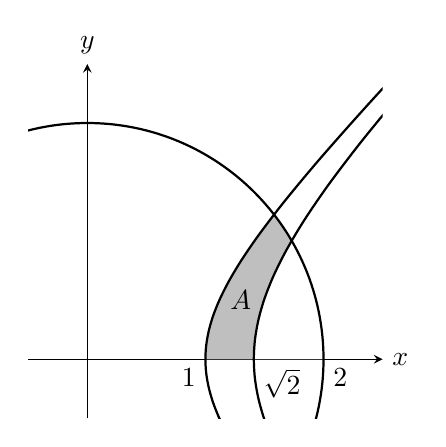
\begin{tikzpicture}[>=stealth, scale=1.5]
    \draw[->] (-0.5, 0) -- (2.5, 0) node[right] {$x$};
    \draw[->] (0, -0.5) -- (0, 2.5) node[above] {$y$};
    \clip (-0.5, -0.5) rectangle (2.5, 2.5);
    \begin{scope}
      \clip (0, 0) circle (2);
      \fill[gray!50, domain=0:1.4, smooth, variable=\t] (1, 0) -- plot ({sec(\t r)},{tan(\t r)}) -- (2, 3) -- (2, 0) -- cycle;
      \fill[white, domain=0:1.4, smooth, variable=\t] (1, 0) -- plot ({1.41 * sec(\t r)},{1.41 * tan(\t r)}) -- (2, 3) -- (2, 0) -- cycle;
    \end{scope}
    \draw[thick] (0, 0) circle (2);
    \draw[thick, domain=-1.4:1.4, smooth, variable=\t] plot ({sec(\t r)},{tan(\t r)});
    \draw[thick, domain=-1.4:1.4, smooth, variable=\t] plot ({1.41 * sec(\t r)},{1.41 * tan(\t r)});

    \node at (1.3, 0.5) {$A$};
    \node[below right] at (2, 0) {2};
    \node[below right] at (1.41, 0) {$\sqrt{2}$};
    \node[below left] at (1, 0) {1};
  \end{tikzpicture}
  \end{center}

  \textbf{Change of Variables}\par
  We first need to choose our change of variables.
  We have a circle and hyperbolas, so it might be a good idea to try $u = x^2 + y^2$ and $v = x^2 - y^2$.
  With this change of variables, it is fiddly to calculate $\pderiv{x}{u}$, $\pderiv{x}{v}$ etc, and it is much easier to calculate $\pderiv{u}{x}$, $\pderiv{u}{x}$, etc, so we apply \cref{JacobianReciprocal} to yield:
  \[
    \frac{\partial(u, v)}{\partial(x, y)} = \det \begin{pmatrix}
    2x & 2y \\
    2x & -2y \\
    \end{pmatrix} = -8xy
  \]
  thus:
  \[
    J = \frac{\partial(x, y)}{\partial(u, v)} = -\frac{1}{8xy}
  \]

  \textbf{Finding $A'$}\par
  We now need to find the corresponding area $A'$.

  There are a couple strategies to do this, although it is often easiest to find the images of the boundary curves of $A$.
  The left and right boundaries of $A$ correspond to $v = 1$ with $1 < u < 4$ and $v = 2$ with $2 < u  < 4$ respectively.
  The lower boundary corresponds to $u = v$ with $1 < u < 2$, and the upper boundary corresponds to $u = 3$ with $1 < v < 2$.
  Thus we have a bijection between $A$ and $A'$ given by:
  \[
    A' = \{(u, v): 1 < v < 2, v < u < 4\}
  \]
  \begin{center}
  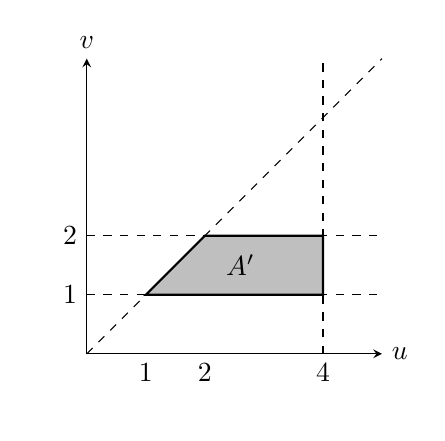
\begin{tikzpicture}[>=stealth, scale=1.5]
    \draw[->] (0, 0) -- (2.5, 0) node[right] {$u$};
    \draw[->] (0, 0) -- (0, 2.5) node[above] {$v$};
    \clip (-0.5, -0.5) rectangle (2.5, 2.5);

    \filldraw[fill=gray!50, draw=black, thick] (0.5, 0.5) -- (1, 1) -- (2, 1) -- (2, 0.5) -- cycle;

    \begin{scope}[dashed]
      \draw (0, 0) -- (2.5, 2.5);
      \draw (2, 0) -- (2, 2.5);
      \draw (0, 0.5) node[left] {1} -- (2.5, 0.5);
      \draw (0, 1) node[left] {2} -- (2.5, 1);
    \end{scope}

    \node at (1.3, 0.75) {$A'$};
    \node[below] at (1, 0) {2};
    \node[below] at (2, 0) {4};
    \node[below] at (0.5, 0) {1};
  \end{tikzpicture}
  \end{center}
  We can also more directly reach this result by considering where the entire $x$-axis, full hyperbolas and full circles map to and then $A'$ must be the unique region enclosed by all four of the images:
  \begin{align*}
    y = 0 &\mapsto u = v \\
    x^2 + y^2 = 4 &\mapsto u = 4 \\
    x^2 - y^2 = 1 &\mapsto v = 1 \\
    x^2 - y^2 = 2 &\mapsto v = 2
  \end{align*}
  \textbf{Computing Integral}\par
  Finally, we can use \cref{areaCoV} to compute the integral:
  \begin{align*}
    \int_{A} x^3y \d{x} &= \int_{A'} x^3y \abs{-\frac{1}{8xy}} \d{u}\d{v} \\
                        &= \frac{1}{8} \int_{A'} \frac{x^3y}{|xy|} \d{u}\d{v} \\
                        &= \frac{1}{8} \int_{A'} x^2 \d{u}\d{v} \text{ as $x , y > 0$} \\
                        &= \frac{1}{8} \int_{A'} \frac{1}{2}(u + v) \d{u}\d{v} \text{ as $u + v = 2x^2$} \\
                        &= \frac{1}{8} \int_{v = 1}^{2} \left(\int_{u = v}^{4} \frac{1}{2}(u + v) \d{u}\right) \d{v} \\
                        &= \frac{1}{16} \int_{1}^{2} (8 + 4v - \frac{3}{2}v^2)\d{v} \\
                        &= \frac{21}{32}
  \end{align*}
\end{example}
\begin{remark}[Advice]
  It is often a good idea to keep $f(x, y)$ in there for as long as possible to see if anything cancels out with the Jacobian before swapping to $u, v$.
\end{remark}
\section{Volume Integrals}
\subsection{Definition}
Volume integrals are fundamentally the same as area integrals, just in a higher dimension.
So to integrate $f(\vec{x}),\ \vec{x} \in \R^3$ over a volume $V \subset \R^3$, we covering $V$ with a large number $N$ of small disjoint subsets $\delta V_i \subset V,\ i \in \{1, \ldots, n\}$ and define:
\[
  \int_{V} f(\vec{x}) \d{V} = \lim_{\Delta \to 0} \sum_{i = 1}^{N} f(\vec{x}_i)\delta V_i
\]
where $\vec{x}_i \in \delta V_i$ and $\Delta$ is the maximum linear dimension of all the $\delta V$, and as $\Delta \to 0$, $N \to \infty$ so that the shrinking volumes still fill the entirety of $V$.

Similarly to area integrals, for reasonable functions, it does not matter how we divide $V$ up, however the obvious way is to use cuboids of volume $\delta x \delta y \delta z$ that are parallel to the axes:
\[
  \int_{x_{\text{min}}}^{x_{\text{max}}} \left(\int_{Y(x)} \left(\int_{Z(x, y)} f(x, y, z) \d{z}\right) \d{y}\right) \d{x}
\]
where $Y(x)$ is the range for each $x$, and $Z(x, y)$ is the range of $z$ for each $x$ and $y$.
Again, similarly to area integrals, we can do the integrals in a different order and still get the same result.
\begin{remark}[Notation]
  Some other notation for $\int_V f(\vec{x}) \d{V}$  include:
  \[
    \int_V f(x, y, z) \d{x} \d{y} \d{z},\ \iiint\limits_V f(x, y, z) \d{V},\ \int_V f(\vec{x}) \d^3{\vec{x}},\ \int\d{x}\int\d{y} \int \d{z} f(x, y, z)
  \]
\end{remark}
\begin{example}[Example Volume Integral]
  Let $V$ be the cuboid $x \in [-a, a],\ y \in [-b, b],\ z \in [-c, c]$.
  Compute $\int_{V} \vec{F} \d{V}$ for $\vec{F} = (z^2, 0, yz)$.

  The recall from \cref{integralVector} that the integral of a vector is just computed by taking component-wise scalar integrals so:
  \[
    \int_{V} \vec{F} \d{V} = \left(\int_{V} z^2 \d{V}, 0, \int_{V} yz \d{V}\right)
  \]
  For the first component, $z^2$ is a separable function so:
  \begin{align*}
    \int_{V} z^2 \d{V} &= \int_{-a}^{a} \int_{-b}^{b} \int_{-c}^{c} z^2 \d{z} \d{y} \d{x} \\
                       &= \int_{-a}^{a} \d{x} \int_{-b}^{b} \d{y} \int_{-c}^{c} z^2 \d{z}  \\
                       &= 2a \cdot 2b \cdot \eval{\frac{1}{3}z^3}{-c}{c} = \frac{8}{3}abc^3
  \end{align*}
  Similarly, for the third component:
  \begin{align*}
    \int_{V} yz \d{V} &= \int_{-a}^{a} 1 \d{x} \int_{-b}^{b} y \d{y} \int_{-c}^{c} z \d{z} \\
                      &= 2a \cdot 2b \cdot \eval{\frac{1}{2}z^2}{-c}{c} = 0
  \end{align*}
  Thus $\int_{V} \vec{F} \d{V} = \frac{8}{3}abc^3(1, 0, 0)$.

  We could have seen that $\int_{V} yz \d{V} = 0$ directly from the symmetry of the cuboid as for each $y \in [-b, b]$, $-y \in [-b, b]$ which has an opposite contribution to the integrand $yz$ and so they cancel out.
\end{example}
\subsection{Change of Variables}
\begin{proposition}[Change of variables for volume integrals]
  If $(u, v, w) \mapsto (x, y, z)$ is a bijection (apart from perhaps at a set of points with measure zero) from a volume $V'$ in the $(u, v, w)$-plane to the volume $V$ in the $(x, y, z)$-plane, then:
  \[
    \int_V f(x, y, z) \d{x} \d{y} \d{z} = \int_{V'} F(u, v, w) \abs{\frac{\partial(x, y, z)}{\partial(u, v, w)}} \d{u}\d{v}\d{w}
  \]
  where $F(u, v, w) = f(x(u, v, w), y(u, v, w), z(u, v, w))$ and:
  \[
    J = \frac{\partial(x, y, z)}{\partial(u, v, w)} \equiv \det \begin{pmatrix}
      \pderiv{x}{u} & \pderiv{x}{v} & \pderiv{x}{w} \\
      \pderiv{y}{u} & \pderiv{y}{v} & \pderiv{y}{w} \\
      \pderiv{z}{u} & \pderiv{z}{v} & \pderiv{z}{w} \\
    \end{pmatrix}
  \]
  is called the \textit{Jacobian} of the transformation.
\end{proposition}
\begin{proof}
  Similarly to the proof of \cref{areaCoV}, but instead in 3D, we divide $V$ into small regions between surfaces of constant $u$, constant $v$, and constant $w$.
  In \cref{volumeElements}, we saw that the volume of each volume element is:
  \[
    \d{V} = \abs{\pderiv{\vec{x}}{u} \cdot \left(\pderiv{\vec{x}}{v} \times \pderiv{\vec{x}}{w}\right)}\d{u}\d{v}\d{w} = \abs{\det\left( \pderiv{\vec{x}}{u} \middle\vert \pderiv{\vec{x}}{v} \middle\vert \pderiv{\vec{x}}{w} \right) \d{u}\d{v}\d{w}} = |J| \d{u}\d{v}\d{w}
  \]
  Where $\det(\vec{u}_1 | \vec{u}_2 | \vec{u}_3)$ is the determinant of the matrix with columns $\vec{u}_1$, $\vec{u}_2$, and $\vec{u}_3$.

  The contribution of this particular volume to the sum defining $\int_V f \d{V}$ is therefore $f(\vec{x}(u, v, w))|J| \d{u} \d{v} \d{w} = F(u, v, w) |J| \d{u} \d{v} \d{w}$.
  Integrating over the values of $(u, v, w) \in V'$, we have:
  \[
    \int_V f \d{x} \d{y} \d{z} = \int_{V'} F |J|\d{u} \d{v} \d{w}
  \]
  Integrating all the contributions of $F(u, v, w) \d{V}$ gives the result.
\end{proof}
The reciprocal rule for the Jacobian (\cref{JacobianReciprocal}) also extends to 3D so:
\[
  \frac{\partial(x, y, z)}{\partial(u, v, w)} = \frac{1}{\frac{\partial(u, v, w)}{\partial(x, y, z)}}
\]

The most common changes of variables for volume integrals are to either cylindrical or spherical polar coordinates.
\subsubsection{Jacobian for Cylindrical Polars}
From \cref{cylindricalPolar}:
\[
  \vec{x} = \begin{pmatrix}
  \rho \cos \phi \\
  \rho \sin \phi \\
  z \\
  \end{pmatrix}
\]
The Jacobian for this change of variables is then:
\[
  J = \det \begin{pmatrix}
  \cos \phi & -\rho \sin \phi & 0 \\
  \sin \phi & \rho \cos \phi & 0 \\
  0 & 0 & 1 \\
  \end{pmatrix} = \rho
\]
By definition, $\rho \geq 0$ so $|J| = |\rho| = \rho$.
\subsubsection{Jacobian for Spherical Polars}
From \cref{sphericalPolar}:
\[
  \vec{x} = \begin{pmatrix}
  r \sin \theta \cos \phi \\
  r \sin \theta \sin \phi \\
  r \cos \theta \\
  \end{pmatrix}
\]
The Jacobian for this change of variables is then:
\[
  J = \det \begin{pmatrix}
  \sin \theta \cos \phi & r \cos \theta \cos \phi & -r \sin \theta \sin \phi \\
  \sin \theta \sin \phi & r \cos \theta \sin \phi & r \sin \theta \cos \phi \\
  \cos \theta & -r \sin \theta & 0 \\
  \end{pmatrix} = r^2 \sin \theta
\]
By definition, $\theta \in [0, \pi]$ so $\sin \theta \geq 0$ and thus $|J| = |r^2 \sin \theta| = r^2 \sin \theta$.
\begin{example}[Volume of a Sphere]
  Calculate the volume of the sphere $r \leq R$.

  To find the volume of an object, we just need to integrate 1 over the whole region:
  \begin{align*}
    \int_{r \leq R} 1 \d{V} &= \int_{r = 0}^{R} \int_{\theta = 0}^{\pi} \int_{\phi = 0}^{2\pi} 1 \cdot r^2 \sin \theta \d{r} \d{\theta} \d{\phi} \\
                            &= \int_{0}^{R} r^2 \d{r} \int_{0}^{\pi} \sin \theta \d{\theta} \int_{0}^{2\pi} \d{\phi} \\
                            &= \frac{1}{3}R^3 \cdot 2 \cdot 2\pi = \frac{4}{3}\pi R^3 \\
  \end{align*}
\end{example}
\begin{example}
  Calculate the volume of a sphere of radius $R$ with a cylinder of radius $a$ removed from it where the axis of the cylinder is in the direction $\vec{m}$ and passes through the centre of the sphere.

  We choose the $z$-axis to be along $\vec{m}$ and choose the $x$ and $y$ axes so that they are perpendicular.
  In cylindrical polars the cylinder occupies $\rho \leq a$ and there sphere occupies $\rho^2 + z^2 \leq R^2$.

  Here, integrating in the order $z$, $\phi$, $\rho$ is the most convenient.
  Since we are including $\rho \leq a$, we integrate $\rho$ from $a$ to $T$.
  For a given $\rho$, we integrate over $\phi$ from 0 to $2\pi$ as we still have volume in all directions.
  Finally for a given $\rho$ and $\phi$, we integrate $z$ between the edges of the sphere, i.e. between $-\sqrt{R^2 - \rho^2}$ and $\sqrt{R^2 - \rho^2}$.

  Therefore the volume is given by:
  \[
    \int_{\rho = a}^{R} \int_{\phi = 0}^{2\pi} \int_{z = - \sqrt{R^2 - \rho^2}}^{\sqrt{R^2 - \rho^2}} 1 \cdot \rho \d{z} \d{\phi} \d{\rho} = 2\pi \int_{a}^{R} 2\rho\sqrt{R^2 - \rho^2} \d{\rho} = \frac{4}{3} \pi(R^2 - a^2)^{3/2}
  \]
  To sanity check our answer, if $a = 0$, we obtain the volume of a sphere as we did not remove anything, and if $a = R$, we obtain 0 as we removed the entire sphere.
\end{example}
\section{Classification of Surfaces}
\begin{definition}[Boundary Curve]
  For a surface $S$, its \textit{boundary curve}, denoted $\partial S$ is the ``edge'' of the surface and the surface is said to \textit{span} its boundary curve.
\end{definition}
\begin{definition}[Open and Closed Surfaces]
  A surface $S$ is \textit{open} if it has a boundary curve and is \textit{closed} if it has no boundary curve, that is, $\partial S = \emptyset$.
\end{definition}
\begin{example}
  \begin{enumerate}
    \item The hemispherical shell:
      \[
        H_R = \{\vec{x}: |\vec{x}| = R, z < 0\}
      \]
      is an open surface with boundary curve:
      \[
        \partial H_R = \{\vec{x}: x^2 + y^2 = R^2, z = 0\}
      \]
      i.e. the edge of the surface is a circle on the $(x, y)$-plane of radius $R$.
    \item The spherical shell $S_R = \{\vec{x}: |\vec{x}| = R\}$ is a closed surface as it has no boundary curve.
    \item The surface of a cube is also closed as it has no boundary curve.
  \end{enumerate}
\end{example}
\begin{definition}[Orientable and Non-Orientable Surfaces]
  A surface is \textit{orientable} if it has two distinct sides and it is \textit{non-orientable} if it has one side.
\end{definition}
\begin{remark}
  There are \textbf{no closed non-orientable surfaces} in $\R^3$.
\end{remark}
\begin{remark}[Tricks to classify surfaces]
  \nonexaminable
  We can classify a closed surface using the fact that every straight line intersects the surface an \textbf{even number of times}.
  Note that points where the line just touches the surface but does not pass through are not counted.

  The upshot of this is that if we can construct a line that intersects the surface an odd number of times, then the surface must be open.
\end{remark}
Importantly, a closed orientable surface has a well-defined interior and exterior whereas an open surface does not as there is always a path between any two points that does not need to pass through the surface.

These definitions apply only to surfaces of finite extent.
For surfaces of infinite extent, for example the $(x, y)$-plane in $\R^3$, we will treat them as the limit of a finite surface.
Since a finite proportion of the $(x, y)$-plane is an open surface and is orientable, as we take the limit, the surface becomes the full plane.
\section{Surface Integrals and Flux}
\subsection{Definitons}
Integrating over a 2D surface $S$ embedded in $\R^3$ is performed similarly to an area integral.
We divide $S$ into small subsets $\delta S_i \subset S$ for $i \in \{1, \ldots, N\}$, and define:
\[
  \int_{S} f(\vec{x}) \d{S} = \lim_{\Delta \to 0} \sum_{i = 1}^{N} f(\vec{x}_i)\delta S_i
\]
in exactly the same way as we did with an area integral (\cref{areaIntegrals}).
The key difference is that in this case $\delta S_i$ are \textbf{not necessarily flat} unlike $\delta A_i$ in the area integral.
\begin{remark}[Notation]
  We can also notate $\int_S f(\vec{x}) \d{S}$ as:
  \[
    \iint\limits_S f(\vec{x}) \d{S}
  \]
  and if $S$ is a closed surface we sometimes use:
  \[
    \oiint f(\vec{x}) \d{S}
  \]
\end{remark}
At each point on an orientable surface, there will be two units normals both pointing in opposite directions.
The unit normal is denoted $\vec{n}$ and depends on the position on the surface.
Which normal direction we choose depends on the application as we will see in the next chapter.

\begin{definition}[Flux]
  If $\vec{F}(\vec{x})$ is a vector field, then the  surface integral $\int_{S} \vec{F}(\vec{x}) \cdot \vec{n} \d{S}$ is the \textit{flux} of $\vec{F}$ through $S$.

  This is just a surface integral with $f(\vec{x}) = \vec{F}(\vec{x}) \cdot \vec{n}$.
\end{definition}
\begin{remark}[Notation]
  \label{vectorSurfaceElement}
  We also introduce the notation:
  \[
    \d{\vec{S}} = \vec{n} \d{S}
  \]
  So $\d{\vec{S}}$ is a vector pointing the direction of the surface normal with magnitude equal to the area of the infinitesimal area $\d{S}$.
  So we can also write the flux of $\vec{F}$ through $S$ as $\int_{S} \vec{F} \cdot \d{\vec{S}}$.
\end{remark}
If $S$ is parameterised by $u$ and $v$ then from \cref{surfaceElements} we know the surface normal and surface element:
\[
  \vec{n} = \pm \frac{\pderiv{\vec{x}}{u} \times \pderiv{\vec{x}}{v}}{\abs{\pderiv{\vec{x}}{u} \times \pderiv{\vec{x}}{v}}} \text{ and } \d{S} = \abs{\pderiv{\vec{x}}{u} \times \pderiv{\vec{x}}{v}} \d{u}\d{v}
\]
and so:
\begin{equation}
  \d{\vec{S}} = \vec{n} \d{S} = \pm \pderiv{\vec{x}}{u} \times \pderiv{\vec{x}}{v} \d{u}\d{v} \label{dSFormula}
\end{equation}
\begin{remark}[Warning]
  A common mistake is to think that $\d{S}$ is just $\d{u} \d{v}$, however this is not true since $\d{S}$ is the area of a parallelogram with sides $\pderiv{\vec{x}}{v} \d{v}$ and $\pderiv{\vec{x}}{u}\d{u}$ and not the area of a flat rectangle in the $(u, v)$-plane.
\end{remark}
Using these results, we can reduce a surface integral to an area integral in the flat $(u, v)$-plane.
\subsection{Examples}
\begin{example}[Surface Area of Shell]
  Find the surface area of the hemispherical shell $H_R = \{\vec{x}: |\vec{x}| = R, z < 0\}$.

  We can use the parameterisation of $H_R$ from \cref{hemisphericalParameterisation}:
  \[
    \vec{x}(\theta, \phi) = \begin{pmatrix}
    R \sin \theta \cos \phi \\
    R \sin \theta \sin \phi \\
    R \cos \theta \\
    \end{pmatrix} \quad \theta \in (\pi/2, \pi], \phi \in [0, 2\pi)
  \]
  We now need to find $\d{S}$:
  \[
    \pderiv{\vec{x}}{\theta} \times \pderiv{\vec{x}}{\phi} = R \begin{pmatrix}
    \cos \theta \cos \phi \\
    \cos \theta \sin \phi \\
    -\sin \theta \\
    \end{pmatrix} \times R \begin{pmatrix}
    -\sin \theta \sin \phi \\
    \sin \theta \cos \phi \\
    0 \\
    \end{pmatrix} = R^2 \begin{pmatrix}
    \sin^2 \theta \cos \phi \\
    \sin^2 \theta \sin \phi \\
    \sin \theta \cos \theta \\
    \end{pmatrix}
  \]
  and so:
  \[
    \d{S} = \abs{\pderiv{\vec{x}}{\theta} \times \pderiv{\vec{x}}{\phi}} \d{\theta} \d{\phi} = R^2 \sin \theta \d{\theta} \d{\phi}
  \]
  We can now integrate 1 over the surface to find its area:
  \begin{align*}
    \int_{H_R} 1 \d{S} &= \int_{\theta = \pi/2}^{\pi} \int_{\phi = 0}^{2\pi} R^2 \sin \theta \d{\theta} \d{\phi} \\
                       &= R^2 \int_{0}^{2\pi} \d{\phi}  \int_{\pi/2}^{\pi} \sin \theta \d{\theta} \\
                       &= R^2 \cdot 2\pi \cdot 1 = 2 \pi R^2
  \end{align*}
\end{example}
\begin{example}[Flux Through a Sphere]
  Find the flux of the vector field:
  \[
    \vec{F}(\vec{x}) = \frac{\alpha}{|\vec{x}|^3} \vec{x}
  \]
  where $\alpha$ is a constant through the surface of the sphere $S_R = \{\vec{x}: |\vec{x}| = R\}$, choosing the normal that points away from the origin.

  We can again parameterise the surface using $\theta$ and $\phi$ but instead with $\theta \in [0, \pi]$ and $\phi \in [0, 2\pi]$.
  Because we use the same parameterisation, we can reuse the result for $\pderiv{\vec{x}}{\theta} \times \pderiv{\vec{x}}{\phi}$ from the previous example and so:
  \[
    \d{\vec{S}} = R^2 \sin \theta \begin{pmatrix}
    \sin \theta \cos \phi \\
    \sin \theta \sin \phi \\
    \cos \theta \\
    \end{pmatrix} \d{\theta} \d{\phi}
  \]
  Note that we take the $+$ sign as this this is the normal which points away from the origin.
  Hence:
  \begin{align*}
    \vec{F} \cdot \d{\vec{S}} &= \frac{\alpha}{R^3} \vec{x} \cdot R^2 \sin \theta \begin{pmatrix}
    \sin \theta \cos \phi \\
    \sin \theta \sin \phi \\
    \cos \theta \\
    \end{pmatrix} \d{\theta} \d{\phi} \\
                              &= \frac{\alpha}{R^3} \begin{pmatrix}
    R \sin \theta \cos \phi \\
    R \sin \theta \sin \phi \\
    R \cos \theta \\
    \end{pmatrix} \cdot R^2 \sin \theta \begin{pmatrix}
    \sin \theta \cos \phi \\
    \sin \theta \sin \phi \\
    \cos \theta \\
    \end{pmatrix} \d{\theta} \d{\phi} \\
                              &= \alpha \sin \theta \d{\theta} \d{\phi}
  \end{align*}
  So calculating the flux:
  \begin{align*}
    \int_{S_R} \vec{F} \cdot \d{\vec{S}} &= \int_{\phi = 0}^{2\pi} \int_{\theta = 0}^{\pi} \alpha \sin \theta \d{\theta} \d{\phi}  \\
                                         &= \alpha \int_{0}^{2\pi} \d{\phi} \int_{0}^{\pi} \sin \theta \d{\theta} \\
                                         &= \alpha \cdot 2\pi \cdot 2 \\
                                         &= 4 \pi \alpha
  \end{align*}
\end{example}
\begin{example}[Flux Through an Infinite Plane]
  Find the flux of $\vec{F}(\vec{x}) = (y^2 e^{-(y^2 + z^2)}, e^{-y^4}, -x^2 e^{-(y^2 + z^2)})$ through the infinite plane $\Pi = \{\vec{x} : x - z = 0\}$ where the normal points in the direction of positive $x$.

  We can parameterise the plane using $x$ and $y$ so that $\vec{x} = (x, y, x)$ since $x = z$.

  We can then find the surface normals:
  \[
    \pderiv{\vec{x}}{x} \times \pderiv{\vec{x}}{y} = \begin{pmatrix}
    1 \\
    0 \\
    1 \\
    \end{pmatrix} \times \begin{pmatrix}
    0 \\
    1 \\
    0 \\
    \end{pmatrix} = \begin{pmatrix}
    -1 \\
    0 \\
    1 \\
    \end{pmatrix}
  \]
  For the normal to point in the positive $x$ direction we need to negate this, and so $\d{\vec{S}} = (1, 0, -1) \d{x} \d{y}$.

  Integrating to find the flux, we have:
  \begin{align}
    \int_{\Pi} \vec{F} \cdot \d{\vec{S}} &= \int_{-\infty}^{\infty} \int_{-\infty}^{\infty} \left[\begin{pmatrix}
        y^2 e^{-(y^2 + z^2)} \\
        e^{-y^4} \\
        -x^2 e^{-(y^2 + x^2)} \\
        \end{pmatrix} \cdot \begin{pmatrix}
        -1 \\
        0 \\
        1 \\
        \end{pmatrix}\right]\d{x} \d{y} \nonumber \\
                                         &= \int_{-\infty}^{\infty} \int_{-\infty}^{\infty} (x^2 + y^2)e^{-(y^2 + x^2)} \d{x} \d{y} \tag{$\star$} \label{doubleIntegralStar} \\
                                         &= \int_{-\infty}^{\infty} x^2 e^{-x^2} \d{x} \cdot \int_{-\infty}^{\infty} e^{-y^2} \d{y} + \int_{-\infty}^{\infty} e^{-x^2} \d{x} \cdot \int_{-\infty}^{\infty} y^2e^{-y^2} \d{y} \nonumber \\
                                         &= 2 \cdot \frac{\sqrt{\pi}}{2} \cdot \sqrt{\pi} = \pi \nonumber
  \end{align}
  We can also more efficiently calculate the integral in \cref{doubleIntegralStar} by transforming into plane polars $(r, \theta)$.
  Noting that $|J| = r$, we have:
  \begin{align*}
    \int_{-\infty}^{\infty} \int_{-\infty}^{\infty} (x^2 + y^2)e^{-(x^2 + y^2)} \d{x} \d{y} &= \int_{0}^{\infty} \int_{0}^{2\pi} r^2 e^{-r^2} \cdot r \d{\theta} \d{r} \\
                                                                                            &= 2\pi \int_{0}^{\infty} r^3 e^{-r^2}\d{r} \\
                                                                                            &= 2\pi \left[\cancelto{0}{\eval{-\frac{1}{2}r^2e^{-r^2}}{0}{\infty}} + \int_{0}^{\infty} re^{-r^2} \d{r}\right] \\
                                                                                            &= 2\pi \eval{-\frac{1}{2}e^{-r^2}}{0}{\infty} \\
                                                                                            &= 2\pi \cdot \frac{1}{2} = \pi
  \end{align*}
\end{example}
\begin{remark}[Warnng]
  We could have calculated the normal of the plane $\vec{n}$ geometrically.
  The plane $\Pi$ is equivalently $\{\vec{x}: \vec{x} \cdot (1, 0, -1) = 0\}$ so $\vec{n} = \left(\frac{1}{\sqrt{2}}, 0, - \frac{1}{\sqrt{2}}\right)$.

  So we might have tried to use:
  \[
    \d{\vec{S}} = \vec{n} \d{S} = \left(\frac{1}{\sqrt{2}}, 0, -\frac{1}{\sqrt{2}}\right) \d{x}\d{y}
  \]
  This however, is not correct, because the area of a surface element is not just $\d{x}\d{y}$.
\end{remark}
\subsection{Useful Results}
\subsubsection{Spherical Surfaces}
\label{sphericalSurfaceVector}
When taking the surface integral over a sphere of constant radius $R$, we have:
\[
  \vec{n} = \frac{\pderiv{\vec{x}}{\theta} \times \pderiv{\vec{x}}{\phi}}{\abs{\pderiv{\vec{x}}{\theta} \times \pderiv{\vec{x}}{\phi}}} = \begin{pmatrix}
  \sin \theta \cos \phi \\
  \sin \theta \sin \phi \\
  \cos \theta \\
  \end{pmatrix} = \frac{1}{R} \vec{x} = \vec{e}_r
\]
This is unsurprising as the outward normal on a sphere is clearly just an outward vector at that point.

Furthermore, the vector surface element with outward normal is:
\[
  \d{\vec{S}} = R^2 \sin \theta \vec{e}_r \d{\theta} \d{\phi}
\]
\subsubsection{Cylindrical Surfaces}
Similarly if we are integrating over the surface of a cylinder of constant radius $a$ then:
\[
  \pderiv{\vec{x}}{\phi} \times \pderiv{\vec{x}}{z} = \begin{pmatrix}
  -a \sin \phi \\
  a \cos \phi \\
  0 \\
  \end{pmatrix} \times \begin{pmatrix}
  0 \\
  0 \\
  1 \\
  \end{pmatrix} = a \begin{pmatrix}
  \cos \theta \\
  \sin \theta \\
  0 \\
  \end{pmatrix} = a e_{\rho}
\]
and so:
\[
  \vec{n} = \frac{\pderiv{\vec{x}}{\phi} \times \pderiv{\vec{x}}{z}}{\abs{\pderiv{\vec{x}}{\phi} \times \pderiv{\vec{x}}{z}}} = \frac{a e_{\rho}}{\rho}  = \vec{e}_\rho
\]
This is clearly an outwards normal on a cylinder.

Furthermore, the vector surface element with outward normal is:
\[
  \d{\vec{S}} = a \vec{e}_\rho \d{\phi} \d{z}
\]
\end{document}
